\subsubsection{Neurons}
The term "neural network" was originally used to describe the workings of nervous systems of animals. These systems consist of a net of neurons that are intricately connected by synapses. These connections carry electrical pulses between the different neurons that can excite them if they exceed certain thresholds, which vary from neuron to neuron and change over time. For example the excitability immediately after activation is almost zero. When this excitation occurs, new pulses in turn propagate through the connections of the excited neuron. Mathematical analyses of these systems have been done as early as the 1940's.\cite{A_logical_calculus_of_the_ideas_immanent_in_nervous_activity}\\
The artificial neural networks that we use for machine learning are inspired by those biological networks. The neurons in our case are mathematical entities that take a fixed number of scalar values as inputs and convert them into a single output value. For a more visual explanation let's take a look at \cref{fig:Neuron_explanation} for the simple case of a 2-input neuron. 
\begin{figure}
	\centering
	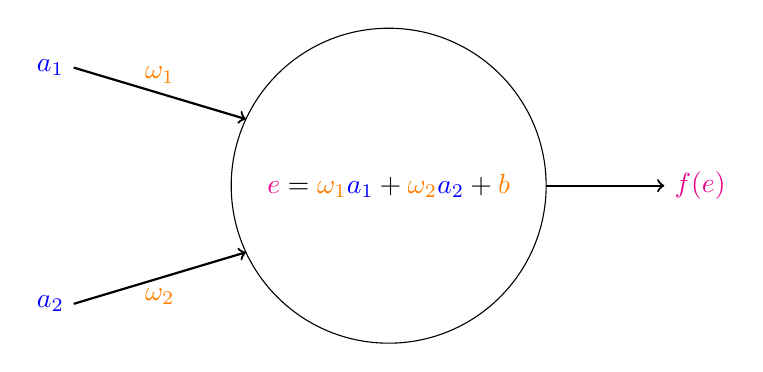
\begin{tikzpicture}[shift={(0,0)}]
	\draw (5,5) circle[radius=2];
	
	% Calculate the coordinates on the circle's circumference
	\pgfmathsetmacro\arrowOneX{5 + cos(155) * 2} % 45 degrees angle
	\pgfmathsetmacro\arrowOneY{5 + sin(155) * 2}
	
	\pgfmathsetmacro\arrowTwoX{5 + cos(-155) * 2} % 135 degrees angle
	\pgfmathsetmacro\arrowTwoY{5 + sin(-155) * 2}
		
	\draw[->, thick] (1,6.5) -- (\arrowOneX, \arrowOneY) node[pos=0.5,above] {$\textcolor{orange}{\omega_1}$};
	\draw (1,6.5) node[left] {$\textcolor{blue}{a_1}$};
	\draw[->, thick] (1,3.5) -- (\arrowTwoX, \arrowTwoY) node[pos=0.5,below] {$\textcolor{orange}{\omega_2}$};
	\draw (1,3.5) node[left] {$\textcolor{blue}{a_2}$};
	\node at (5,5) {$\textcolor{magenta}{e} = \textcolor{orange}{\omega_1}\textcolor{blue}{a_1} + \textcolor{orange}{\omega_2}\textcolor{blue}{a_2} + \textcolor{orange}{b}$};	
	\draw[->, thick] (7,5) -- (8.5,5) node[right] {$\textcolor{magenta}{f(e)}$};
	
	
\end{tikzpicture}
	\caption{This figure explains the general operating principle of neurons in neural networks as they are used in this thesis. The parameters are denoted in orange, the input activations in blue and the activation with its corresponding activation function in green.}
	\label{fig:Neuron_explanation}
\end{figure}
The big circle in the middle is representing what we consider a neuron. It takes as input the activation values $a_i$, multiplies them with their corresponding weights $\omega_i$, sums them up, adds a bias value $b$ and then applies the activation function to get the resulting output value. The input activations $a_i$ correspond to the electronic pulses in the nerve system, with the strength of the pulse coded into the value itself. No pulse in the biological system would be represented by an activation of zero in the mathematical model. The weights $\omega_i$ are a representation of how important single input values are for the activation of the neuron itself. In the biological counterpart this might correspond to how thick or conductive the connections between the nerve cells are. Finally, the combination of bias $b$ and activation function describes how high the sum of the input-weight-pairs has to be to activate the neuron and how the resulting value for the activation of the neuron changes for higher input activations. For example, a very simple output activation function would be a heaviside function. The neuron then outputs $1$ if the sum of the input-weight-pairs is bigger than the negative bias $-b$ and a 0 otherwise. Hence the neuron can only be on or off. A more common activation function that will be used for the rest of this thesis is the ReLU function (Rectified Linear Unit). This function is defined as 
\begin{equation}
	f(x) = 
	\begin{cases}
		x, &\text{if } x\geq0 \\
		0, &\text{otherwise}
	\end{cases}.
\end{equation}
Here the neuron gets activated as soon as the sum of the input-weight-pairs is higher than $-b$ and the value of the activation increases linearly with the weighted input summation.
\subsubsection{Neural networks}
A neural network can be built from these neurons, by connecting the outputs of certain neurons to the inputs of others. For example lets consider a neural network that consists of 3 layers of 4 neurons each, that takes 2 values as an input and outputs 2 values at the end. This could for example be trained for detecting if a point on a 2d-grid is inside or outside of a given region. The input values would be the $x$ and $y$ coordinates of the point and the output value could represent the probability of the point being inside the desired region. How exactly this training would work will be explained in later chapters. A visual sketch of such a network can be seen in \cref{fig:Neural_network_example}. \\
\begin{figure}
	\centering
	\begin{tikzpicture}
	\Vertex[x=0,y=0]{A}
	\Vertex[x=0,y=1]{B}
	\Vertex[x=0,y=2]{C}
	\Vertex[x=0,y=3]{D}
	
	\Vertex[x=2,y=0]{E}
	\Vertex[x=2,y=1]{F}
	\Vertex[x=2,y=2]{G}
	\Vertex[x=2,y=3]{H}
	
	\Vertex[x=4,y=0]{I}
	\Vertex[x=4,y=1]{J}
	\Vertex[x=4,y=2]{K}
	\Vertex[x=4,y=3]{L}
	
	\Edge[lw=1pt](A)(E)
	\Edge[lw=1pt](A)(F)
	\Edge[lw=1pt](A)(G)
	\Edge[lw=1pt](A)(H)
	
	\Edge[lw=1pt](B)(E)
	\Edge[lw=1pt](B)(F)
	\Edge[lw=1pt](B)(G)
	\Edge[lw=1pt](B)(H)
	
	\Edge[lw=1pt](C)(E)
	\Edge[lw=1pt](C)(F)
	\Edge[lw=1pt](C)(G)
	\Edge[lw=1pt](C)(H)
	
	\Edge[lw=1pt](D)(E)
	\Edge[lw=1pt](D)(F)
	\Edge[lw=1pt](D)(G)
	\Edge[lw=1pt](D)(H)
	
	\Edge[lw=1pt](E)(I)
	\Edge[lw=1pt](E)(J)
	\Edge[lw=1pt](E)(K)
	\Edge[lw=1pt](E)(L)
	
	\Edge[lw=1pt](F)(I)
	\Edge[lw=1pt](F)(J)
	\Edge[lw=1pt](F)(K)
	\Edge[lw=1pt](F)(L)
	
	\Edge[lw=1pt](G)(I)
	\Edge[lw=1pt](G)(J)
	\Edge[lw=1pt](G)(K)
	\Edge[lw=1pt](G)(L)
	
	\Edge[lw=1pt](H)(I)
	\Edge[lw=1pt](H)(J)
	\Edge[lw=1pt](H)(K)
	\Edge[lw=1pt](H)(L)
	
	\Vertex[x=-2,y=1, label=$x$, opacity = 0]{X}
	\Vertex[x=-2,y=2, label=$y$, opacity = 0]{Y}
	\Edge[lw=1pt](X)(A)
	\Edge[lw=1pt](X)(B)
	\Edge[lw=1pt](X)(C)
	\Edge[lw=1pt](X)(D)
	\Edge[lw=1pt](Y)(A)
	\Edge[lw=1pt](Y)(B)
	\Edge[lw=1pt](Y)(C)
	\Edge[lw=1pt](Y)(D)
	
	\Vertex[x=6,y=1.5, label=$p$, opacity = 1]{P}
	\Edge[lw=1pt](I)(P)
	\Edge[lw=1pt](J)(P)
	\Edge[lw=1pt](K)(P)
	\Edge[lw=1pt](L)(P)
	
	\draw [decorate,
	decoration = {brace, mirror, amplitude=10pt}] (-0.2,-0.5) --  (4.2,-0.5);
	\node at (2,-1.2) {3 (hidden) layers};
	\draw [decorate,
	decoration = {brace, mirror, amplitude=10pt}] (6.5,-0.3) --  (6.5,3.3);
	\node at (7.2,1.5) [rotate=-90] {width of 4 neurons};
	
\end{tikzpicture}
	\caption{This figure shows an example of a neural network. It consists of multiple neurons connected to each other. This specific network has 2 input values and one output value. The names of those input and output values correspond to the use case of identifying if a 2d point lies within a region in 2d space.}
	\label{fig:Neural_network_example}
\end{figure}
This network is only a very specific example of what a neural network might look like. In reality, there are various kinds of networks used to learn different tasks. For this thesis we will only talk about "fully connected" or "dense" neural networks. This means that every neuron in the first layer will receive every possible input value, and every neuron in later layers will receive the output of every neuron in the previous layer as an input. How the output gets handled may still differ through different use cases. The structure of a neural network is generally called the architecture of the network. 